\section{Case Study 1: SIR}
- maps nicely to continuous time-semantics and state-transitions provided by FRP
- STM results in considerable performance boost

The implementation of the susceptible, infected and recovered agents are the same except that instead of accessing the environment through \textit{get} and \textit{put}, we use \textit{readTVar}, \textit{writeTVar} and \textit{modifyTVar}.

We checked the visual outputs and the dynamics and they look qualitatively the same to the reference implementation. Summarizing the performances:
\begin{center}
  \begin{tabular}{ l || c }
    Implementation & Avg. Duration \\ \hline \hline 
    State Monad & 101.15 sec \\ \hline
   	STM Single-Core & 52.75 sec \\ \hline
   	STM 4-Core & 20.57 sec 
  \end{tabular}
\end{center}

When we scale up the grid-size for the 4-core version we get the following results (single run in each case, gives only a rough estimate): 
\begin{center}
  \begin{tabular}{ c || c }
    Grid-Size & Duration \\ \hline \hline 
    51 x 51 & 21 sec \\ \hline
    101 x 101 & 92 sec \\ \hline
    151 x 151 & 188 sec \\ \hline
    201 x 201 & 305 sec \\ \hline
    251 x 251 & 530 sec 
    
    \label{tab:agent_by_duration_stm}
  \end{tabular}
\end{center}

Further we investigated how well STM scales to multiple cores by running the 51 x 51 on 1-4 cores:
\begin{center}
  \begin{tabular}{ c || c }
    Cores & Duration \\ \hline \hline 
    1 & 52 sec \\ \hline
    2 & 28 sec \\ \hline
    3 & 22 sec \\ \hline
    4 & 21 sec
    
    \label{tab:cores_by_duration_stm}
  \end{tabular}
\end{center}

\subsubsection{Comparison to IO implementation}
We also implemented the same model running in the IO Monad and doing the synchronisation all 'manually' aquiring and releasing the locks explicitly. In this case, the environment is shared using an IOVar and the access is synchronised using an MVar. We get the following performance (single run in each case, gives only a rough estimate):
\begin{center}
  \begin{tabular}{ c || c }
    Grid-Size & Duration \\ \hline \hline 
    51 x 51 & 38 sec \\ \hline
    101 x 101 & 158 sec \\ \hline
    151 x 151 & 370 sec \\ \hline
    201 x 201 & 661 sec \\ \hline
    251 x 251 & 1154 sec 
    
    \label{tab:agent_by_duration_io}
  \end{tabular}
\end{center}

The Figure \ref{fig:agent_by_duration} clearly indicates that STM outperforms the low level IO implementation by a substantial factor and scales much smoother.
\begin{figure}
	\centering
	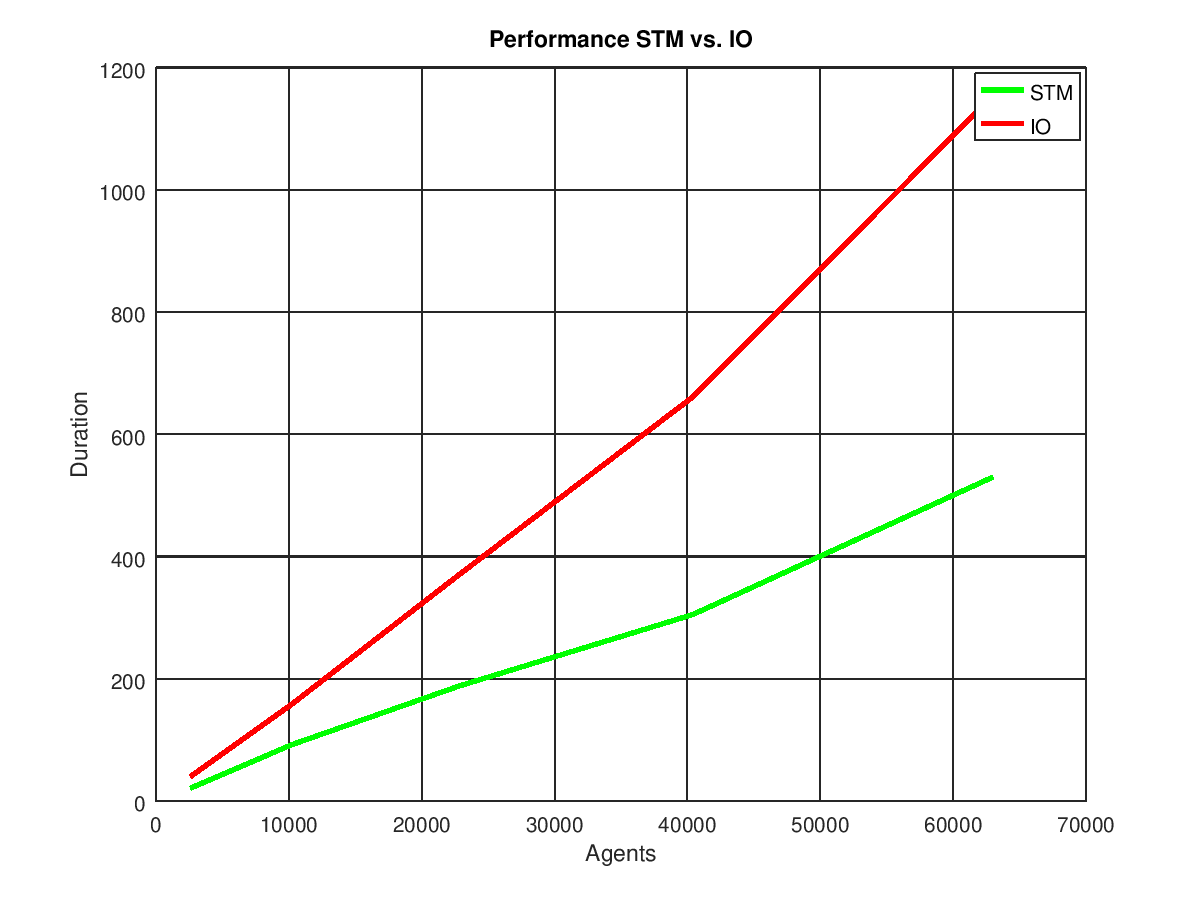
\includegraphics[width=0.6\textwidth, angle=0]{./fig/agents_duration_stm_io.png}
	\caption{Comparison of STM (Table \ref{tab:agent_by_duration_stm}) and IO performance (Table \ref{tab:agent_by_duration_io})}
	\label{fig:agent_by_duration}
\end{figure}

Further we investigated how well IO scales to multiple cores by running the 51 x 51 on 1-4 cores (single run in each case, gives only a rough estimate):
\begin{center}
  \begin{tabular}{ c || c }
    Cores & Duration \\ \hline \hline 
    1 & 61 sec \\ \hline
    2 & 45 sec \\ \hline
    3 & 40 sec \\ \hline
    4 & 38 sec
    
    \label{tab:cores_by_duration_io}
  \end{tabular}
\end{center}

Comparing the scaling to multiple cores of the IO (Table \ref{tab:cores_by_duration_io}) and STM implementation (Table \ref{tab:cores_by_duration_stm}) shows no significant difference between STM and IO as can be seen in Figure \ref{fig:core_duration_stm_io}.

\begin{figure}
	\centering
	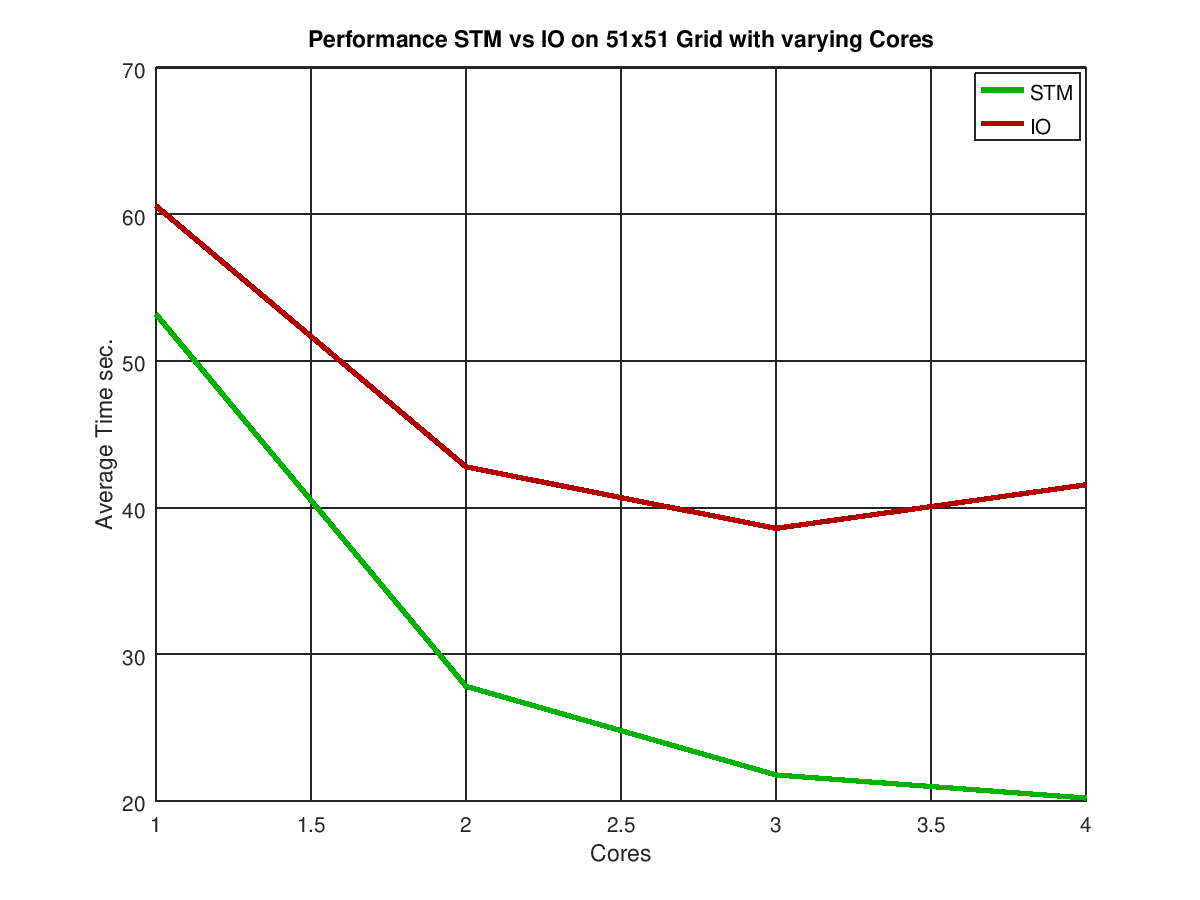
\includegraphics[width=0.6\textwidth, angle=0]{./fig/core_duration_stm_io.png}
	\caption{Comparison of scaling IO (Table \ref{tab:agent_by_duration_stm}) and STM  (Table \ref{tab:agent_by_duration_stm}) to multiple cores.}
	\label{fig:core_duration_stm_io}
\end{figure}

\subsubsection{Comparison to Java RePast single core}
To have an idea where the functional implementation is performance-wise compared to the established object-oriented methods, we conducted a performance comparison with a Java implementation using RePast, running on a single-core. All parameters were the same and the simulation was run until virtual time t=100 was reached, on various grid-sizes. Due to the lack of proper timing facilities in RePast we measured the time by hand using a stopwatch. Although this is not very precise it gives a rough estimate and allows a very basic comparison, being precise enough if the difference is larger than 1 second. We measured the following:

\begin{center}
  \begin{tabular}{ l || c | r }
    Grid-Size & Java Repast & 4-Core Haskell \\ \hline \hline 
    51 x 51 & 10 sec & 20 sec \\ \hline
    101 x 101 & 110 sec & 92 sec \\ \hline
    201 x 201 & 1260 sec & 305 sec \\ \hline
    
    \label{tab:agent_by_duration_repast}
  \end{tabular}
\end{center}

As can be seen in Figure \ref{agent_by_duration_repast}, while on a 51x51 grid the single-core Java RePast version outperforms the 4-core Haskell STM version by about 200\%, the figure is inverted on a 201x201 grid where the 4-core Haskell STM version outperforms the single core Java Repast version by 400\%. We can conclude that the single-core Java RePast version clearly outperforms the Haskell STM 4-core version on small grid-sizes but that the Haskell STM version scales up with increasing grid-sizes and clearly outperforms the RePast version with increasing number of agents.

\begin{figure}
	\centering
	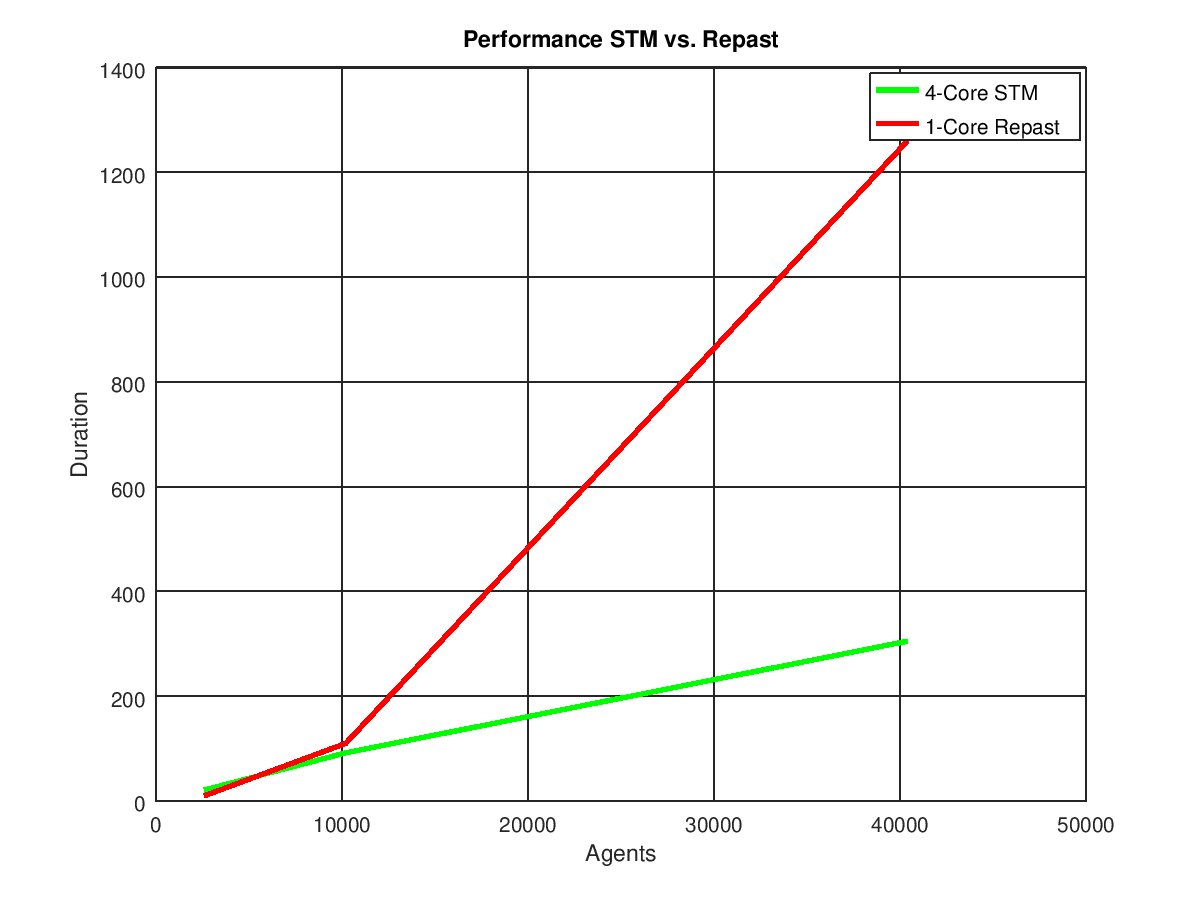
\includegraphics[width=0.6\textwidth, angle=0]{./fig/agents_duration_stm_repast.png}
	\caption{Comparison of 4-Core STM and single core Repast (Table \ref{tab:agent_by_duration_repast}).}
	\label{fig:agent_by_duration_repast}
\end{figure}

\subsection{Conclusions}
Interpretation of the performance data leads to the following conclusions:
\begin{enumerate}
	%\item On a single core, no transaction retries should happen, the results support that assumption.
	\item Running in STM and sharing state using a TVar is much more time- and memory-efficient than running in the State Monad.
	\item Running STM on multiple cores concurrently leads to a significant performance improvement (for that model).
	\item STM outperforms the low level locking implementation, running in the IO Monad, substantially and scales much smoother.
	\item Both STM and IO show same scaling performance on multiple cores, with the most significant improvement when scaling from a single to 2 cores.
	\item STM on single core is still slower than an object-oriented Java implementation on a single core.
	\item STM on multiple cores dramatically outperforms the single-core object-oriented Java implementation on a single core on instances with large agent numbers.
\end{enumerate}